
\begin{itemize}
    \item 
\item  $N-free-model-parameters << N-constraints$
\item  In our specific design this expands to:
\item  $(model parameters + current-injection-value-parameter) << N (independent and uncorrelated)$ constraints.
\item  For the different classes of Reduced Model we show that the optimizer converges when data is simulated.


Here I show graphs of
\end{itemize}



In a simulated experiment, existing models were instantiated using a randomly chosen model parameters.

In the class of reduced neural models we are optimizing, are not arbitrary waveform generators. The models have intrinsic restrictions that prevent them from matching perfectly with experimental waveforms.

When constraints are derived from model measurements, intrinsic model restrictions no longer apply. Optimized models should match perfectly with the simulated experiments. 

* Failure to match is indicative of: -- Failure to setup tractable optimization problems. Too higher a dimension.

- When inverting linear equations, finding a unique solution requires that the number of constraining equations is greater than the number of free variables you are solving for:

\section{Pitfalls}
Errors are correlated, and constraints are too few.
To protect against a situation where the collection of error sources guiding optimization are too correlated with each other, to act as 


\section{Verification}
Ground truths are model solutions that we know are correct independently from the optimizer. One way to establish ground truths is to identify the global minima by exhaustively searching the solution space. An exhaustive search is a reasonable approach when you consider only one or two model parameters are free parameters, however if one does 100 samples in each of N dimensions then one must make samples $100^{N}$ total samples to be sure of ehaustively searching, assuming the most efficient code, hardware and development time $N=3$, may be the highs.  Also the choice of 100 samples is nominal, 100 samples could be either too fine or too sparse, depending on how if the parameter being searched exhibits 2nd order sensitivity.

It is more computationally efficient to obtain ground truths by simulating constraining data using digital models. It is easy to simulate constraining data, all that is required is that you take a neuronal model and measure its behavior in response to carefuly chosen current injection values. Measured behavior can then be used to construct NeuronUnit tests, were the measurements become "observations", or observed behaviors. To make the simulated data cover a range of circumstances, one can make different NU measurements by randomly choosing different parameter values of models to find.

It was important to be able to establish ground truths that were always possible for the optimizer to match exactly. Often experimental data implies waveform shapes that are beyond the capabilities of the model that is to be fitted. Simulating experimental measurements meant, that model limitations can be understood separately from optimizer limitations.

\section{Optimizer Limitations}


\begin{center}
    \begin{figure}
    
        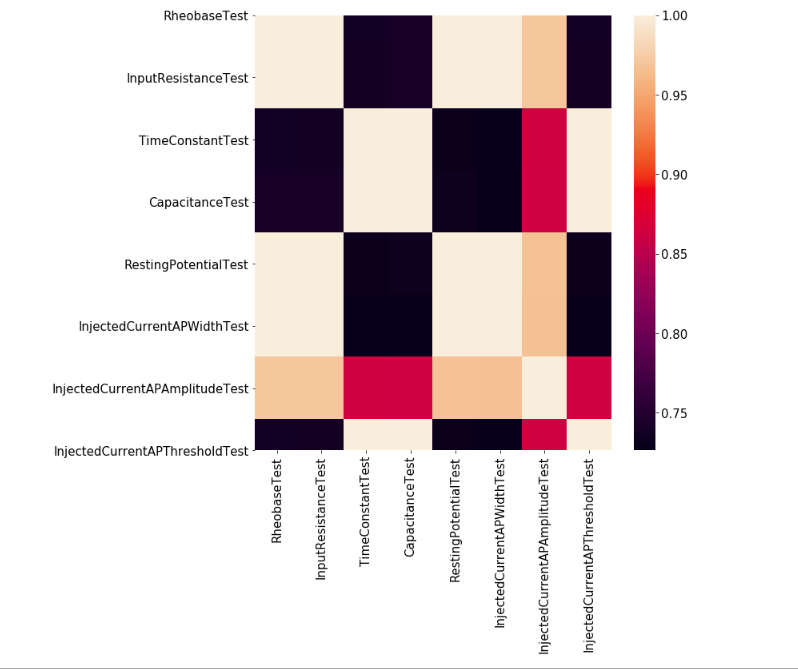
\includegraphics[width=\linewidth]{figures/correlated_errors.png}
    
    	\caption{Test caption}
    \end{figure}
\end{center}